\chapter{Introduction}\label{ch:introduction}

Aircraft engine overhaul is the process of removing, disassembling, inspecting, repairing, cleaning, reassembling and testing a used engine. Overhaul involves the intricate process of taking an engine apart, and in doing so, undoing up to thousands of small parts from the engine—eg. screws, nuts and bolts. In order to reassemble the engine in the overhaul process, the small parts have to be sorted and classified. Figure \ref{fig:unclassified_small_parts} shows an example of small parts that need to be classified.

\begin{figure}[H]
\centering
\makebox[\textwidth][c]{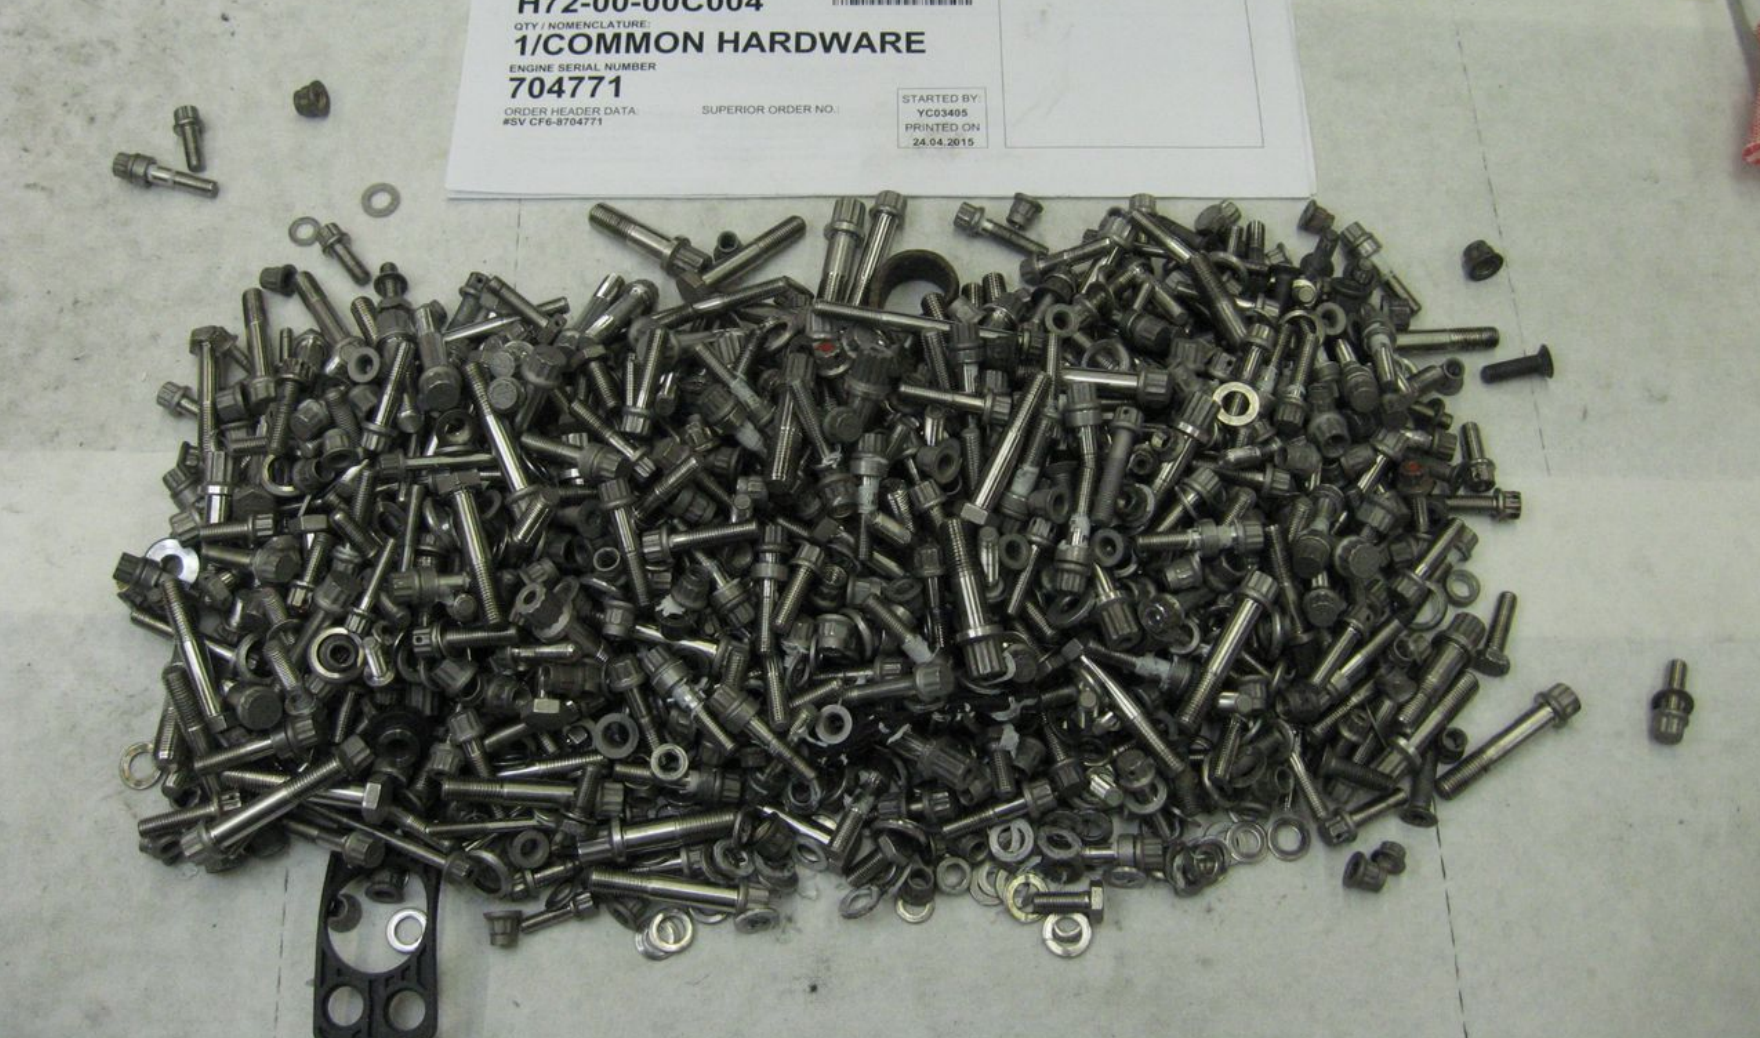
\includegraphics[width=0.65\textwidth]{unclassified_small_parts}}
\caption{Small parts that were taken apart during an aircraft engine overhaul, and have to be sorted for reassembling.}
\label{fig:unclassified_small_parts}
\end{figure}

\subsubsection{Manual Small Part Classification}

Traditionally, the tasks of classifying and sorting small parts are executed manually by a human task force. The dismantled small parts are brought to the workers in a special work station, where the workers have access to manuals, pictures of each small part, magnifiers and measuring instruments. The small parts are engraved with a part number which can be used for identification. However, sometimes the part number is indistinguishable due to erosion, rust or physical damage. In this case, the workers have to look up the small part in the manuals. The measuring instruments are used to compute the small part's distinguishing features as shown in \ref{fig:small_part_structure}. For classifying a small part with a distorted part number, the workers might need a few seconds to measure the different small part features and compare them against the models in the manual for classification. The time can varry depending on the small part and the exprience of the worker.

\begin{figure}[H]
\centering
\makebox[\textwidth][c]{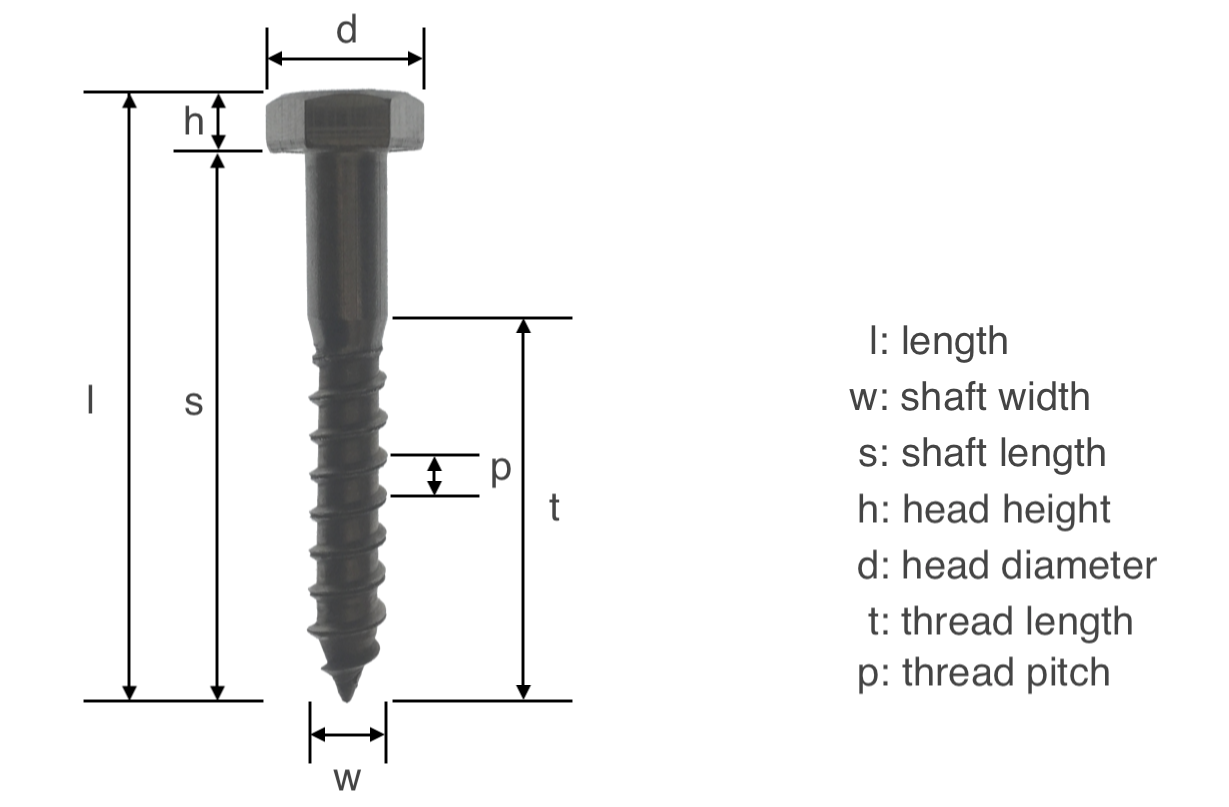
\includegraphics[width=0.85\textwidth]{small_part_structure}}
\caption{The structure of a sample screw displaying the different associated measurements.}
\label{fig:small_part_structure}
\end{figure}

\subsubsection{Automatic Small Part Classification}

An automatic small part classification system involves a setup where a camera and a robotic arm are placed over a conveyor belt. First, the small parts are placed on the conveyor belt. Next, the camera takes pictures of the small parts that are rolling underneath on the conveyor belt. The pictures are then sent to an image classification system which in turn classifies the images of the small parts. The classification system sends the labels of the small parts to the robotic arm, which uses those labels to sort the small parts accordingly. Figure \ref{fig:automatic_system} shows the automatic small part classification system.

The main brain behind automatic small part classification is the image classification system. In order to build a small part image classification system, we employ convolutional neural networks (CNNs). CNNs have become the state-of-the-art approach to classical computer vision and image processing tasks such as image classification, object detection and many others \cite{ILSVRC15}.

The automatic approach involves minimal human interaction, and thus slashes the amount of man power required to sort and classify small parts. Moreover our automatic approach provides a quantifiable measurement for accuracy which can be used to assess and improve the classification system.

\begin{figure}[H]
\centering
\makebox[\textwidth][c]{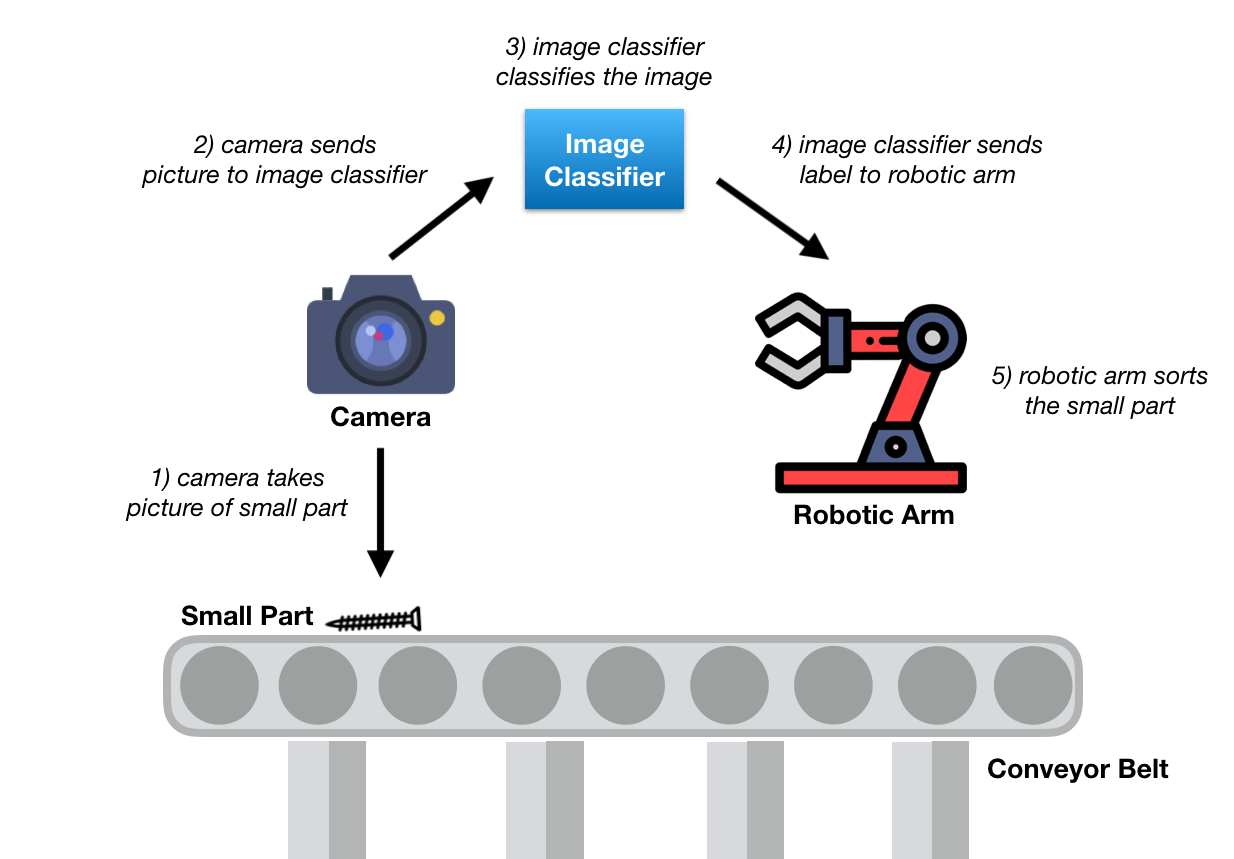
\includegraphics[width=0.9\textwidth]{automatic_system}}
\caption{The automatic small part classification system.}
\label{fig:automatic_system}
\end{figure}


\section{Problem}

Convolutional neural networks are characteristically data-centric algorithms. The performance of a CNN algorithm depends on the availability of a dataset of images that can capture each target object's intra-class variability \cite{krizhevsky2012imagenet}. In our case, we need to train a convolutional neural network using images that capture the distinguishing features of each of our small parts. Since aircraft engines can have up to thousands of small parts, and our CNN requires multiple images of each small part, the task of collecting an image set can be time consuming.

Our contribution in this thesis is twofold. 1) we describe a system to generate synthetic images for the classification of small parts. In addition to using pictures of the small parts, we obtain their respective 3D models and use 3D modeling software to render 2D synthetic images of the small parts. The advantage being that the images are rendered rather than collected manually using a camera, and hence generation of the output image set requires less time and effort. 2) we train a convolutional neural network using synthetic images. We assess the use of synthetic data as input for CNN algorithms to perform image classification. We explore the use of a fully synthetic dataset and also a mixed dataset of both real and synthetic images in different ratios.

\section{Motivation}

Using synthetic images to classify small objects yields the power of convolutional neural network while overcoming the need to collect and annotate a dataset of images manually. This approach is extendable to image classification problems in other novel domains.

Furthermore, the process of generating synthetic images gives full control of the surrounding environment to the creator of the synthetic scene. The 3D models and the synthetic scenes can be easily adjusted to capture specific differentiating features of the small parts.

\section{Outline}
In chapter \ref{ch:background}, convolutional neural networks are described and the necessary mathematical background needed to navigate this thesis is provided. We also define the terminology that we use to describe small parts and different types of images in our dataset. Chapter \ref{ch:related_work} transcribes the literature that was reviewed in preparation for this thesis. A review of convolutional neural networks based image classification, image classification in industrial use cases and the usage of synthetic data is provided. In chapter \ref{ch:analysis}, the requirements of our system are broken down. The system use cases, object model and deployment diagrams are presented. In chapter \ref{ch:system_design}, we describe our subsystems and the relationships between them. We also describe the software and hardware components used for implementation. Chapter \ref{ch:object_design} provides an in-depth explanation of the external frameworks, APIs, algorithms and software that we use out-of-the-box. Chapter \ref{ch:evaluation} contains our implementation details, experiment design and results. Lastly, chapter \ref{ch:summary} contains a recap of our work, the conclusions we have reached and the potential future work that can be based on our thesis.
